\documentclass{homework}

\title{Problem Set 1}
\author{Kevin Evans}
\studentid{11571810}
\date{January 26, 2021}
\setclass{Physics}{463}
\usepackage{amssymb}
\usepackage{mathtools}
\usepackage{graphicx}
\usepackage{amsthm}
\usepackage{amsmath}
\usepackage{slashed}
\usepackage{boldline}
\usepackage{physics}
\usepackage{tcolorbox}
\usepackage[inter-unit-product =\cdot]{siunitx}

\usepackage[makeroom]{cancel}
\usepackage{booktabs}
\usepackage{multirow}

\usepackage{times}
\usepackage{mhchem}
\usepackage{enumitem}
\usepackage[normalem]{ulem}
\usepackage{systeme}
\usepackage{tikz}
\usepackage{mathtools}
\usepackage{tabularx}


\newcommand{\fm}{\femto\meter}

\begin{document}
	\maketitle
	\begin{enumerate}
		\item % 1.1
			Given two vectors $\bvec{a}_1$ and $\bvec{a}_2$ from Fig. 10, \begin{align*}
				\bvec{a}_1 & = \frac{1}{2} a\left(\uvec{x} + \uvec{y} - \uvec{z}\right) \\
				\bvec{a}_2 & = \frac{1}{2} a \left(-\uvec{x} + \uvec{y} + \uvec{z}\right),
			\end{align*}
			the angles between these can be found using the inner product, \begin{align*}
				\bvec{a}_1 \cdot \bvec{a}_2 & = \frac{a^2}{4} \left(-1 + 1 - 1\right) = -\frac{a^2}{4} \\
					& = a_1 a_2 \cos \theta. \\
				\cos \theta & = -\frac{a^2}{4} \left(\frac{2}{a\sqrt{3}}\right)^2 = \frac{1}{3} \\
				\Aboxed{ \theta & \approx \SI{70.53}{\deg}. }
			\end{align*}
		
		\item % 1.2
			From Figure 11, the $(100)$ plane intercepts the $x$ and $z$ axis at $\sqrt{2}a$. Normalizing this, the new plane is $(100)$.
			
			For $(001)$, it's similar but intercepts the $y$ and $z$ axis, leading to $(011)$.
		
		\item A single \ce{NaCl} molecule will have a volume \begin{align*}
			\SI{23}{\atomicmassunit} \times \SI{1.660e-27}{\kg \per \atomicmassunit} \times \SI{1000}{\g \per \kg} / \SI{1.0}{\g \per \centi\meter\cubed} & = \SI{3.82e-23}{\centi\meter\cubed} \\
				& = a^3 \\
			\Aboxed{ \implies a & = \SI{3.37}{\angstrom}. }
		\end{align*}
	
		\item % 1/6 pi
			For \underline{simple cubic}, the spheres will have radius $a/2$. Using a volume of a sphere, \begin{align*}
				V_\mathrm{sph} & = \frac{4}{3} \pi \left(\frac{a}{2}\right)^3 \\
					& = \frac{a^3}{6} \pi \\
				\text{Packing fraction }  P & = \frac{V_\mathrm{sph}}{V_\mathrm{cube}} \\
					& = \frac{1}{6} \pi. 
			\end{align*}
			
			For \underline{body-centered cubic}, the spheres will have radius $\sqrt{3}a/4$ (from the listed nearest neighbor distance, halved to give radius) and there will be two full spheres. The volume is then \begin{align*}
				V_\mathrm{sph} & = 2 \times \frac{4}{3} \pi \left(\sqrt{3}a/4\right)^3 \\
					& = \frac{\pi \sqrt{3}}{8} a^3. \\
				P & = \frac{\pi \sqrt{3}}{8}.
			\end{align*}
			
			For \underline{face-centered cubic}, the spheres will have radius $a/2\sqrt{2}$ and now there are four full spheres enclosed. \begin{align*}
				V_\mathrm{sph} & = 4 \times \frac{4}{3} \pi \left(\frac{a}{2\sqrt{2}}\right)^3 \\
					& = \frac{\pi \sqrt{2}}{6} a^3. \\
				P & = \frac{\pi \sqrt{2}}{6}.
			\end{align*}
		\item \begin{enumerate}
			\item \ce{ABC3}? I'm not entirely sure.
			\item sc.
			\item \begin{minipage}[t]{0.6\textwidth}
				A primitive lattice translation vectors are just $a$ in each direction, \begin{align*}
					\bvec{a}_1 & = a \uvec{x} \\
					\bvec{a}_2 & = a \uvec{y} \\
					\bvec{a}_3 & = a \uvec{z}.
				\end{align*}
			\end{minipage}
			~ 
			\begin{minipage}[t]{0.4\textwidth}
					\vspace{0.1em}
					\begin{center}
						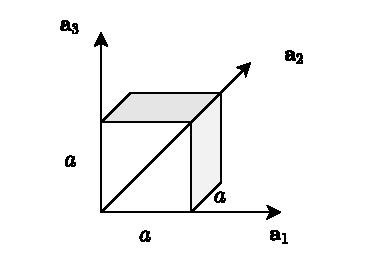
\includegraphics[width=0.9\linewidth]{primcell}
					\end{center}
			\end{minipage}
			
			\item For atom A, there is one atom per cell, \begin{align*}
				\bvec{r}_1 & = 0.
			\end{align*}
			For atom B, there is one atom per cell, \begin{align*}
				\bvec{r}_5 & = 0.5 \bvec{a}_1 + 0.5 \bvec{a}_2 + 0.5 \bvec{a}_3.
			\end{align*}
			For atom C, there are 3 atoms per cell, \begin{align*}
				\bvec{r}_2 & = 0.5 \bvec{a}_1 + 0.5 \bvec{a}_2 \\
				\bvec{r}_3 & = 0.5 \bvec{a}_1 + 0.5 \bvec{a}_3 \\
				\bvec{r}_4 & = 0.5 \bvec{a}_2 + 0.5 \bvec{a}_4.
			\end{align*}
		\end{enumerate}
	\end{enumerate}
\end{document}